\documentclass[a4paper]{article}
\usepackage[utf8]{inputenc}
\usepackage{polski}
\usepackage{graphicx}
\usepackage{listings}
\usepackage{placeins}
\usepackage{amssymb}
\usepackage{float}
\usepackage{color}
\usepackage{algorithm}
\usepackage[noend]{algpseudocode}
\usepackage[left=2.5cm,right=2.5cm,top=2.5cm,bottom=2.5cm]{geometry}
\usepackage{amsmath}
\usepackage{enumerate}
\usepackage{indentfirst}
\usepackage[demo]{graphicx}
\usepackage{mathtools}

\title{SPC - LAB1}
\author{Paweł Szczepaniak, Marcin Gruchała, Michał Bagiński}
\date{16.10.2020}

\lstset{frame=tb,
  language=Matlab,
  aboveskip=3mm,
  belowskip=3mm,
  showstringspaces=false,
  columns=flexible,
  basicstyle={\small\ttfamily},
  numbers=none,
  numberstyle=\tiny\color{gray},
  keywordstyle=\color{blue},
  commentstyle=\color{dkgreen},
  stringstyle=\color{mauve},
  breaklines=true,
  breakatwhitespace=true,
  tabsize=3
}

\begin{document}

\maketitle

\section{Wstęp}
    Celem ćwiczenia było wyznaczenie odpowiedzi skokowych $\lambda(t)$ obiektu II rzędu o transmitancji
    $$
    K(s)=\dfrac{1}{s^2+as+b}
    $$
    dla różnych przypadków położenia biegunów dla podanych scenariuszy:
        \begin{itemize}
            \item $\Delta > 0$,
            \item $\Delta = 0$,
            \item $\Delta < 0$.
        \end{itemize}
    Gdzie $\Delta = a^2-4b$ 
\section{Schemat układu}
  W zadaniu zbudowaliśmy model symulacyjny w oprogramowaniu SIMULINK. Schemat symulacyjny wykorzystuje blok Transfer Fcn. Blok modeluje transmitancje operatorową systemu w dziedzinie operatora S. 
\begin{figure}[H]
    \centering
    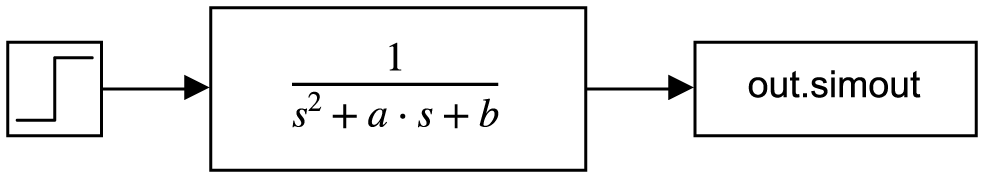
\includegraphics[scale=0.35]{simulink.png}
    \caption{Schemat blokowy rozwiązania}
\end{figure}
\section{Wyniki symulacji}
\subsection{$\Delta > 0$}
\subsubsection{Układ stabilny}
$$
a=3,\quad b=1
$$
\begin{figure}[H]
    \centering
    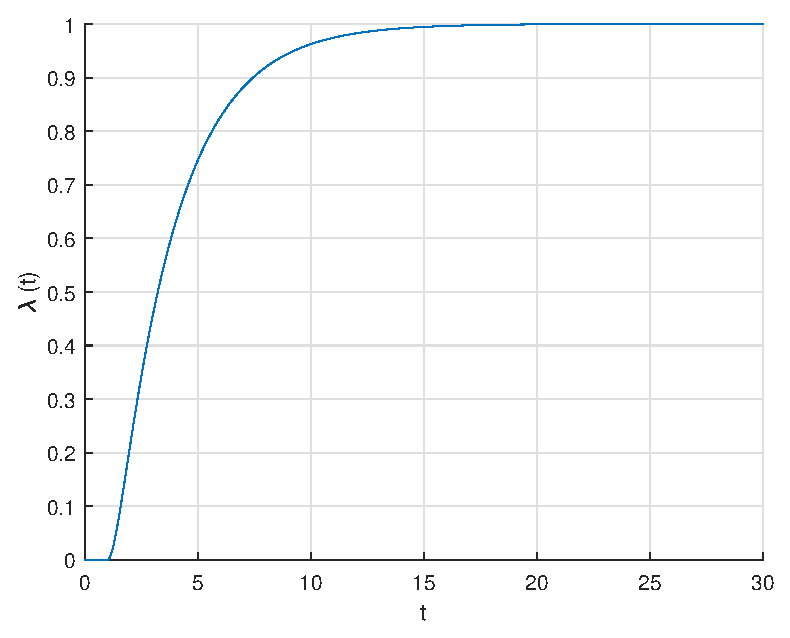
\includegraphics[scale=0.6]{a1.eps}
    \caption{Wykres symulacji układu stabilnego dla $\Delta>0$}
\end{figure}
\begin{figure}[H]
    \centering
    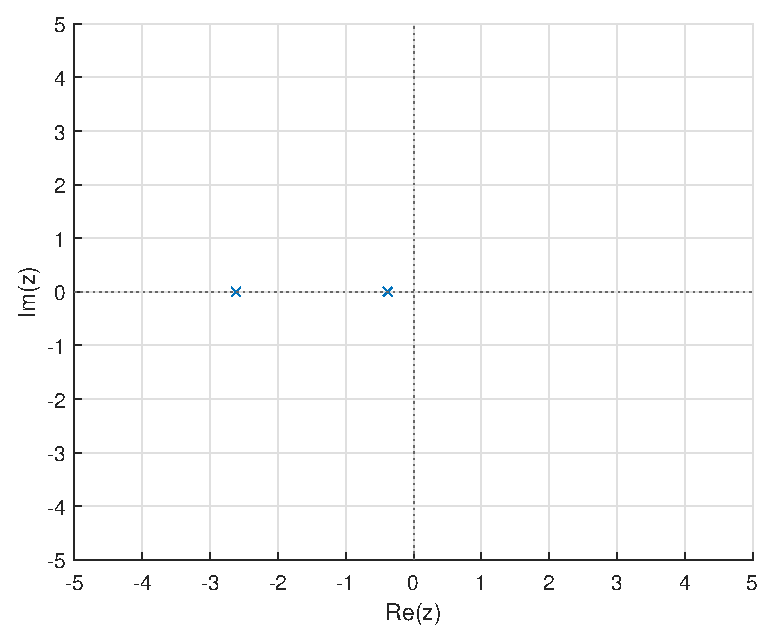
\includegraphics[scale=0.6]{a1_z.eps}
    \caption{Rozkład biegunów transmitancji układu stabilnego dla $\Delta>0$}
\end{figure}
\subsubsection{Układ niestabilny}
$$
a=3,\quad b=-5
$$
\begin{figure}[H]
    \centering
    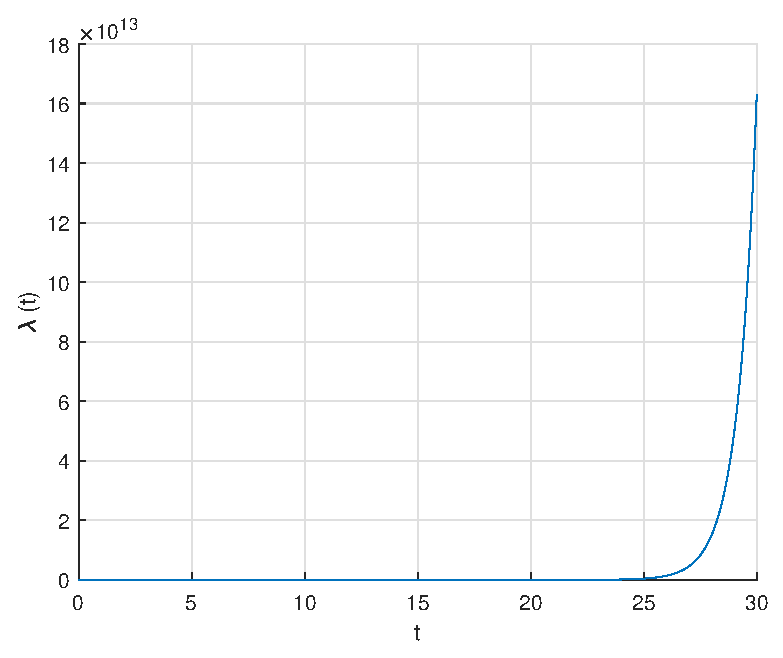
\includegraphics[scale=0.6]{a2.eps}
    \caption{Wykres symulacji układu niestabilnego dla $\Delta>0$}
\end{figure}
\begin{figure}[H]
    \centering
    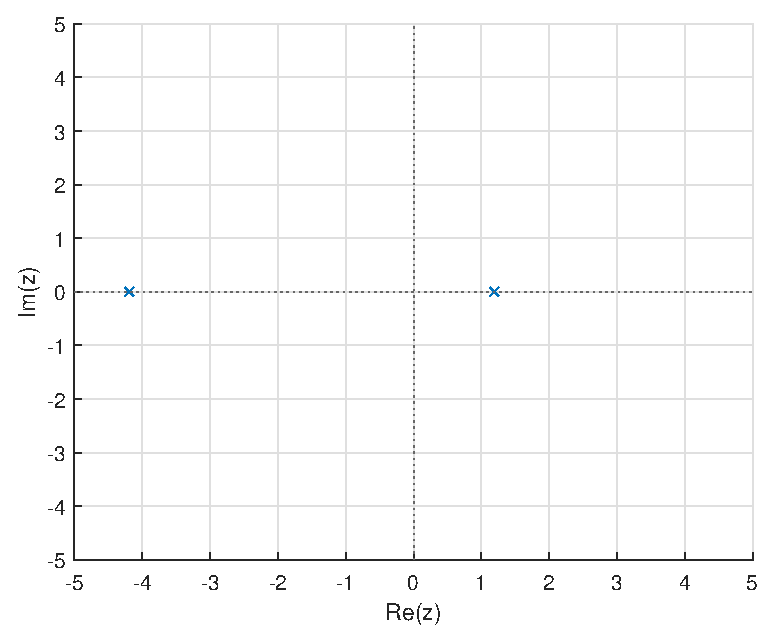
\includegraphics[scale=0.6]{a2_z.eps}
    \caption{Rozkład biegunów transmitancji układu niestabilnego dla $\Delta>0$}
\end{figure}
\subsection{$\Delta = 0$}
\subsubsection{Układ stabilny}
$$
a=2,\quad b=1
$$
\begin{figure}[H]
    \centering
    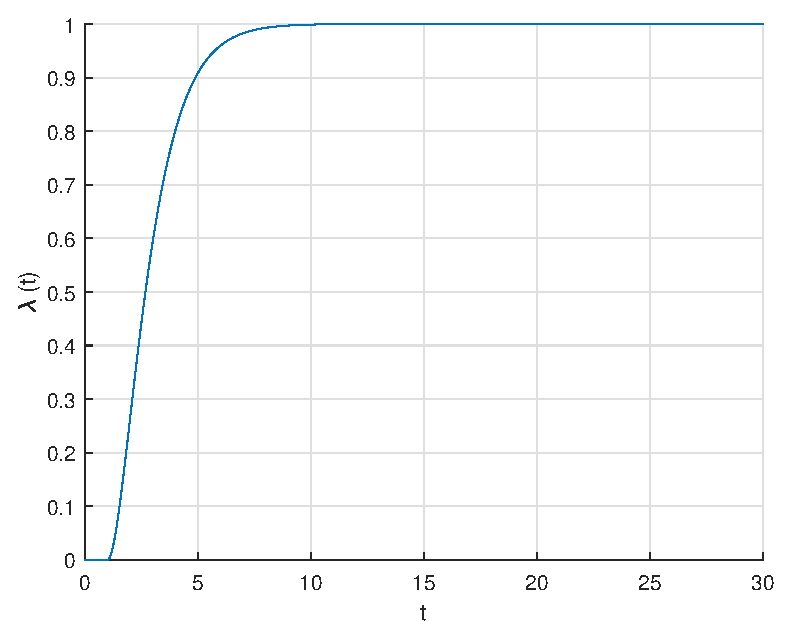
\includegraphics[scale=0.6]{b1.eps}
    \caption{Wykres symulacji układu stabilnego dla $\Delta=0$}
\end{figure}
\begin{figure}[H]
    \centering
    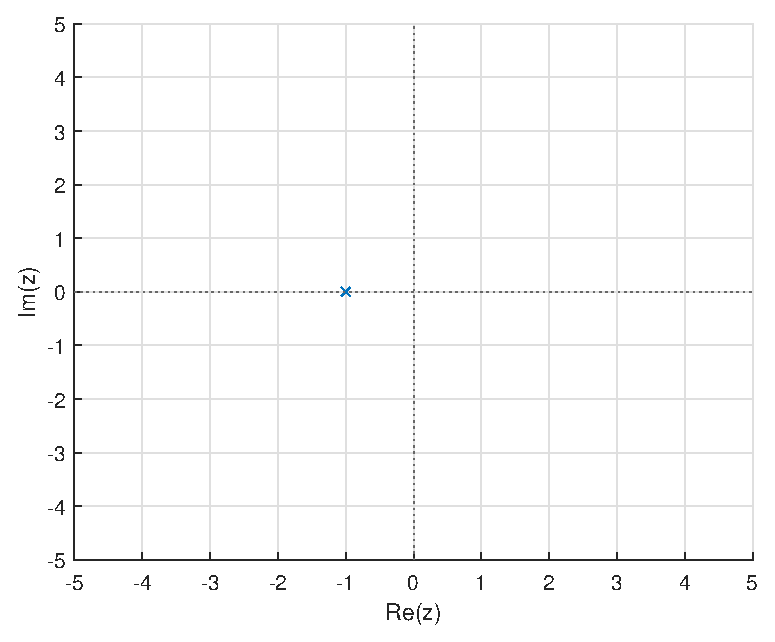
\includegraphics[scale=0.6]{b1_z.eps}
    \caption{Rozkład biegunów transmitancji układu stabilnego dla $\Delta=0$}
\end{figure}
\subsubsection{Układ niestabilny}
$$
a=-4,\quad b=4
$$
\begin{figure}[H]
    \centering
    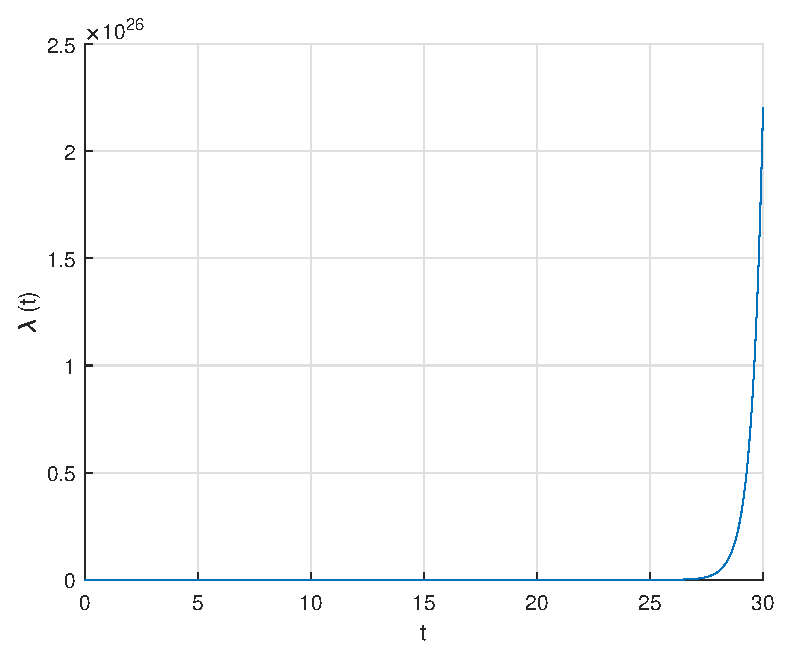
\includegraphics[scale=0.6]{b2.eps}
    \caption{Wykres symulacji układu niestabilnego dla $\Delta=0$}
\end{figure}
\begin{figure}[H]
    \centering
    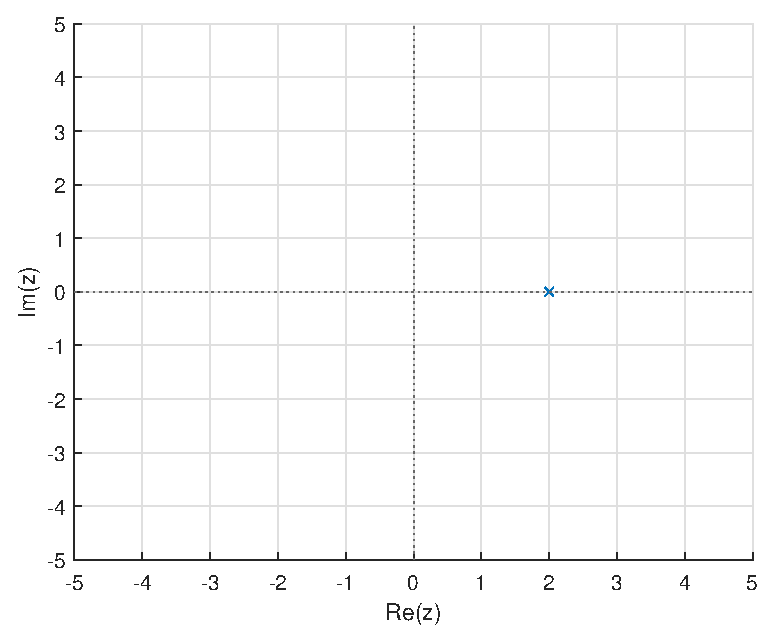
\includegraphics[scale=0.6]{b2_z.eps}
    \caption{Rozkład biegunów transmitancji układu niestabilnego dla $\Delta=0$}
\end{figure}
\subsection{$\Delta < 0$}
\subsubsection{Układ stabilny}
$$
a=1,\quad b=2
$$
\begin{figure}[H]
    \centering
    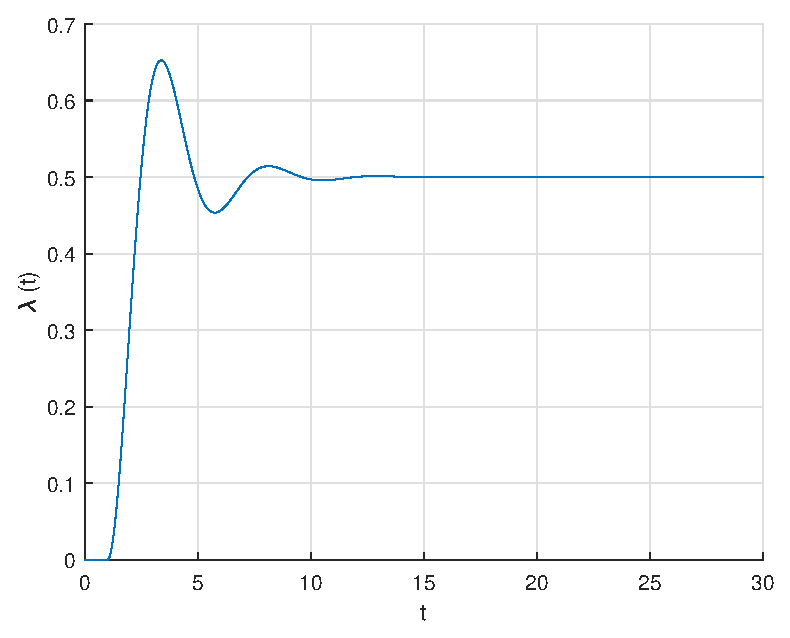
\includegraphics[scale=0.6]{c1.eps}
    \caption{Wykres symulacji układu stabilnego dla $\Delta<0$}
\end{figure}
\begin{figure}[H]
    \centering
    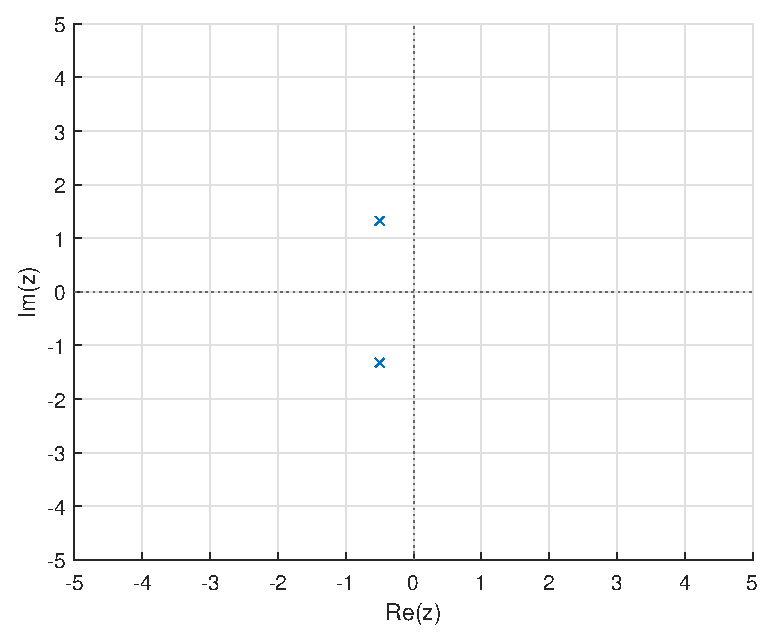
\includegraphics[scale=0.6]{c1_z.eps}
    \caption{Rozkład biegunów transmitancji układu stabilnego dla $\Delta<0$}
\end{figure}
\subsubsection{Układ niestabilny}
$$
a=-1,\quad b=1
$$
\begin{figure}[H]
    \centering
    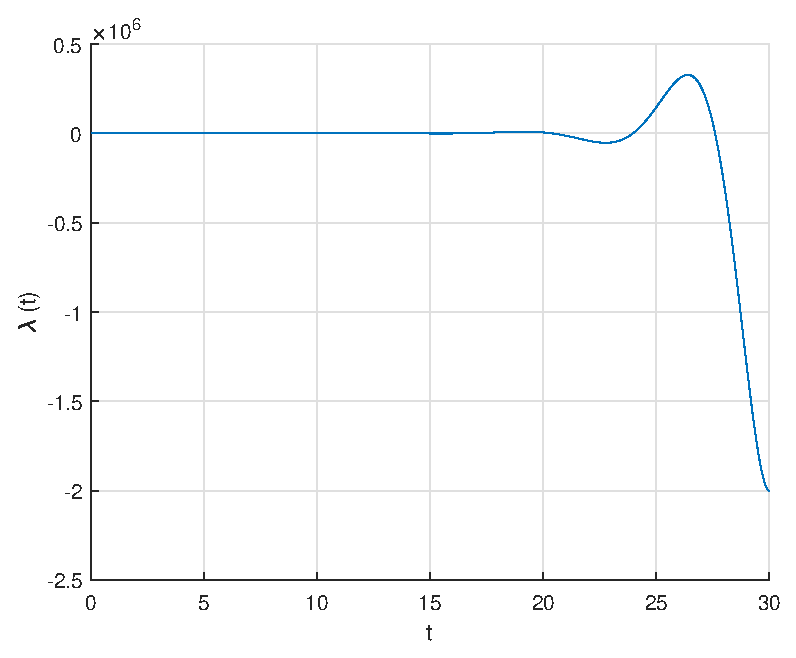
\includegraphics[scale=0.6]{c2.eps}
    \caption{Wykres symulacji układu niestabilnego dla $\Delta<0$}
\end{figure}
\begin{figure}[H]
    \centering
    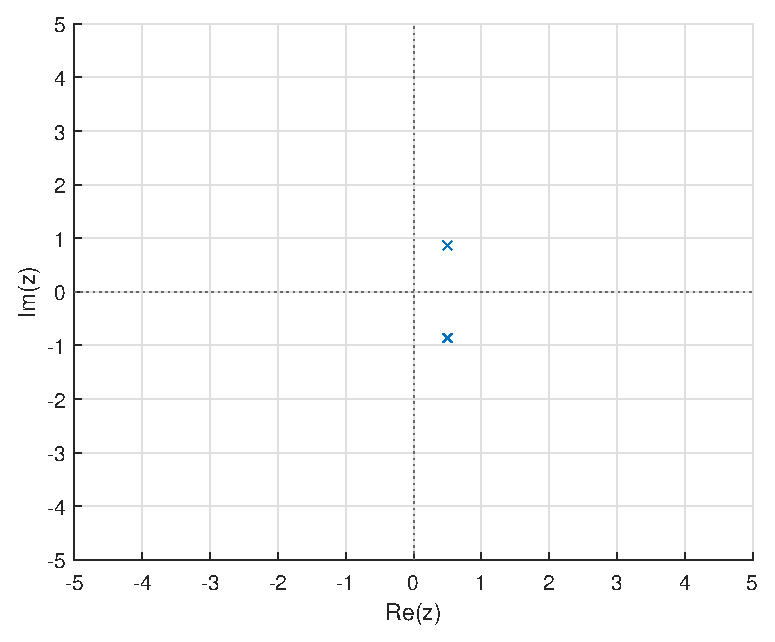
\includegraphics[scale=0.6]{c2_z.eps}
    \caption{Rozkład biegunów transmitancji układu niestabilnego dla $\Delta<0$}
\end{figure}
\section{Kod źródłowy}
\subsection{$\Delta<0$}
\subsubsection{Układ stabilny}
\lstinputlisting[]{lab_a1.m}
\subsubsection{Układ niestabilny}
\lstinputlisting[]{lab_a2.m}
\subsection{$\Delta<0$}
\subsubsection{Układ stabilny}
\lstinputlisting[]{lab_b1.m}
\subsubsection{Układ niestabilny}
\lstinputlisting[]{lab_b2.m}
\subsection{$\Delta<0$}
\subsubsection{Układ stabilny}
\lstinputlisting[]{lab_c1.m}
\subsubsection{Układ niestabilny}
\lstinputlisting[]{lab_c2.m}

\section{Wnioski}
     \subsection{Skok jednostkowy}
       \indent Funkcja skokowa Heaviside'a to nieciągła funkcja przyjmująca wartość 0 dla wszystkich  ujemnych argumentów oraz wartość 1 w przypadku każdego innego argumentu tj. wszystkich liczb  rzeczywistych nieujemnych. \\
        \indent Skok jednostkowy oznacza się często za pomocą symbolu $\boldsymbol{1}(t)$. \\
        \indent Funkcja ta umożliwia uzyskanie charakterystyki skokowej tj. odpowiedzi układu na wymuszenie w postaci skoku jednostkowego przy zerowych warunkach początkowych. Pozwala to na dokonanie podstawowej analizy układu dynamicznego w prosty sposób.
        \subsection{Analiza rezultatów}
            \begin{figure}[H]
                \centering
                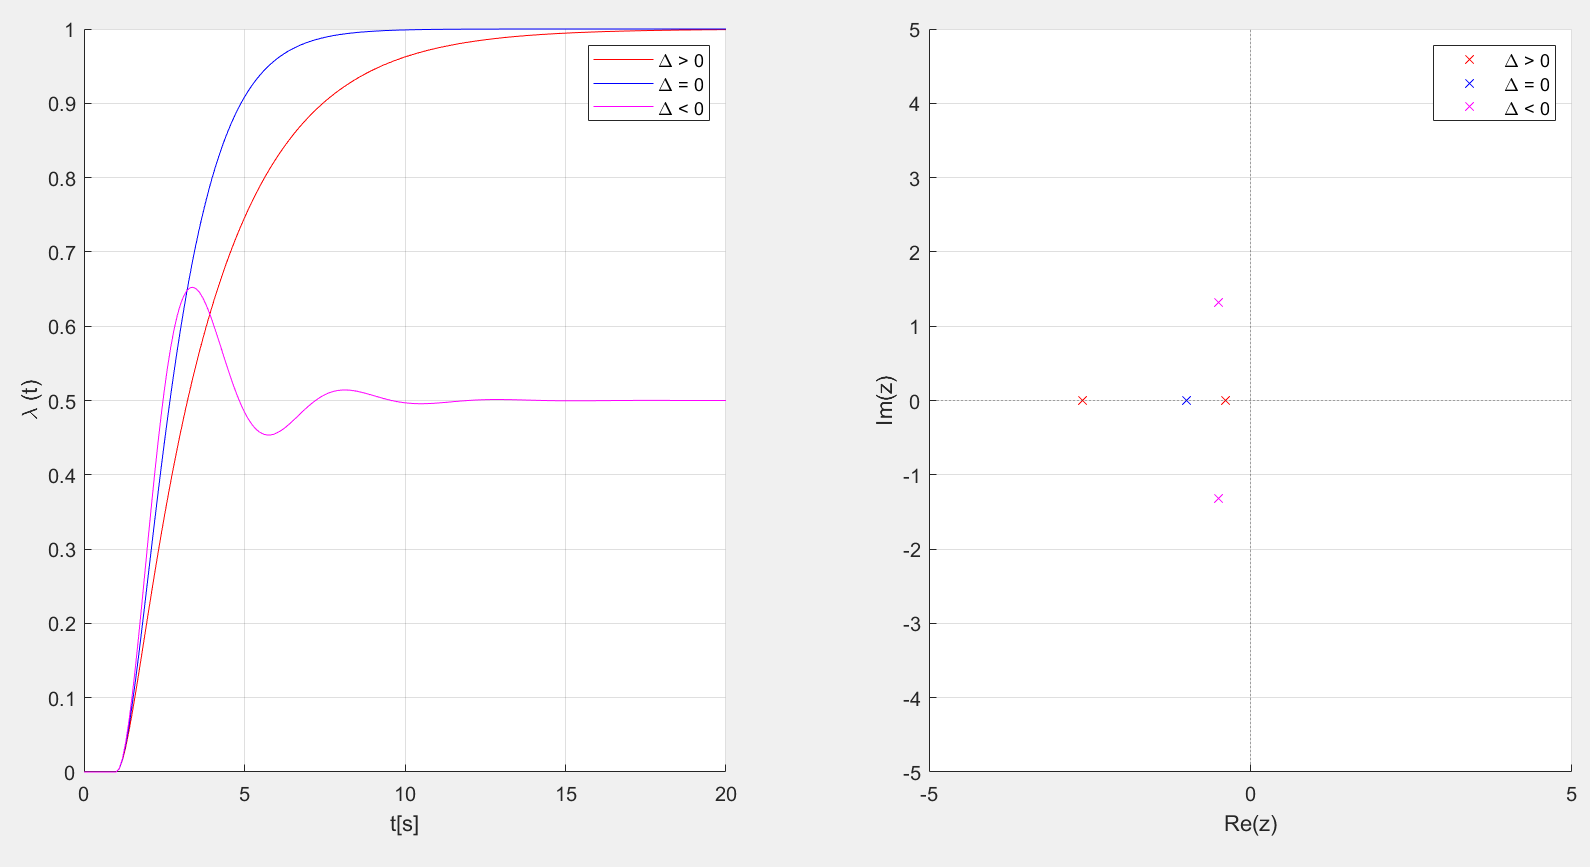
\includegraphics[scale=0.5]{porownianie_odpowiedzi.png}
                \caption{Porównanie odpowiedzi skokowych i położenia pierwiastków na osi zespolonej dla układów stabilnych}
            \end{figure}
            \begin{figure}[H]
                \centering
                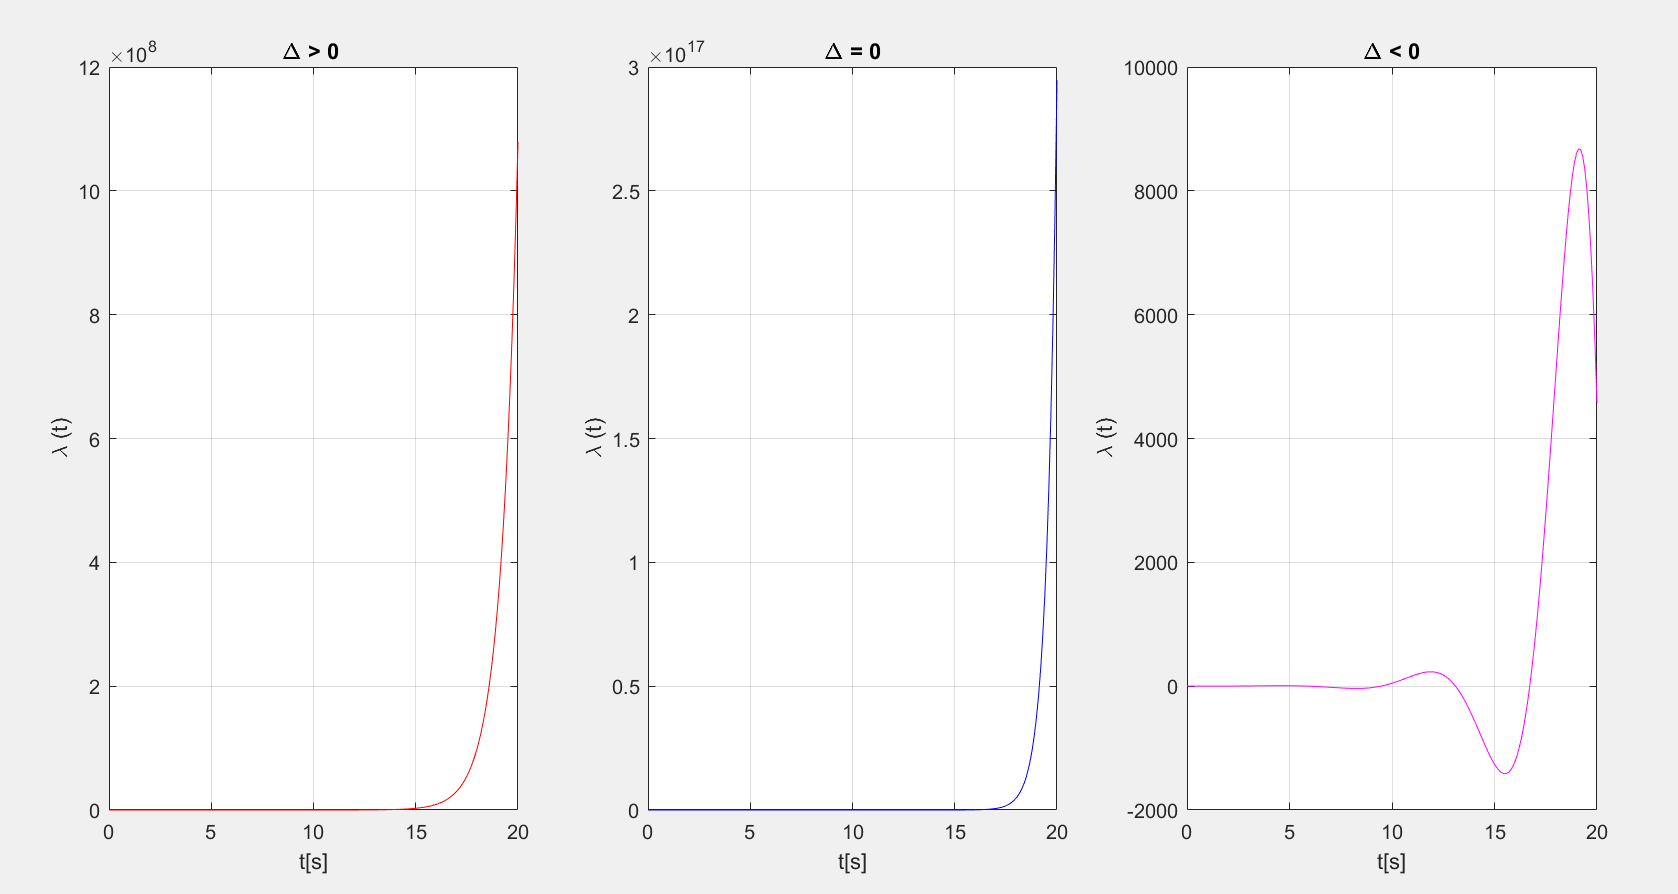
\includegraphics[scale=0.5]{niestabilny_skok.png}
                \caption{Porównanie odpowiedzi skokowych dla układów niestabilnych}
            \end{figure}
            \begin{figure}[H]
                \centering
                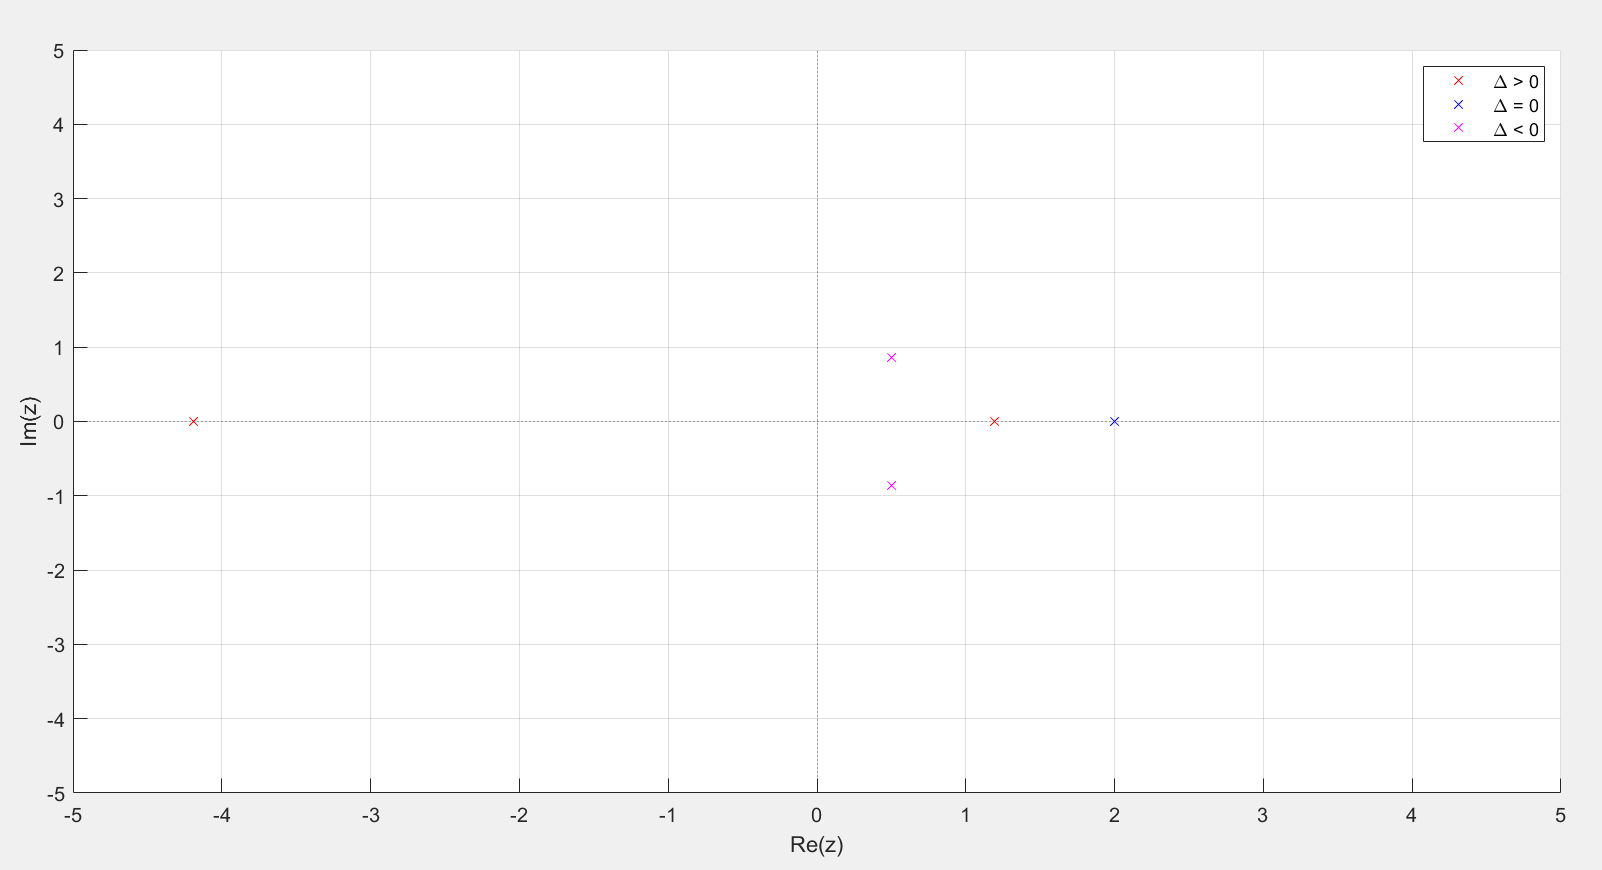
\includegraphics[scale=0.5]{niestabilny_pierwiastki.png}
                \caption{Porównanie położenia pierwiastków układów niestabilnych na osi zespolonej}
            \end{figure}
            Wykresy odpowiedzi skokowej są bardzo przydatne podczas analizy układów, można z nich wywnioskować podstawowe własności układu dynamicznego takie jak stabilność czy czas stabilizacji.    
            Odpowiedz układu na skok jednostkowy jest zależna od pierwiastków mianownika transmitancji opisującej układ. \\
           \indent Aby układ był stabilny pierwiastki mianownika transmitancji muszą się znajdować w lewej półpłaszczyźnie na osi zespolonej. Pojawienie się pierwiastków poza osią liczb rzeczywistych powoduje pojawienie się w układzie oscylacji. Warto zaznaczyć, że w momencie gdy choćby jeden z pierwiastków znajduje się w prawej części osi liczb rzeczywistych tzn. rzeczywista część pierwiastka jest $>$ 0 to układ ten jest niestabilny.  //
           \indent Wyniki doświadczenia potwierdzają wiedzę na temat równania różniczkowego drugiego rzędu, którą posiedliśmy już na wcześniejszych kursach. Zatem jeśli:
           \begin{itemize}
               \item $\Delta < 0$ - w układzie zachodzą przeregulowania, oscylacje,
               \item $\Delta \geq 0$ - układ bez oscylacji,
               \item $Re(\lambda_1), Re(\lambda_2) < 0$ - układ jest stabilny,
               \item $Re(\lambda_1), Re(\lambda_2) > 0$ - układ jest niestabilny.
           \end{itemize}
        
    \section{Realne obiekty}
    Badany model obiektu drugiego rzędu można zastosować do opisu realnych obiektów. Obiekty te aby nadawały się do opisu równaniem różniczkowym drugiego rzędu powinny być zbudowane z co najmniej dwóch elementów magazynujących energię.   
    \newline
    
    Przykłady realnych obiektów spełniające dane równanie:
    \begin{itemize}
        \item amortyzator,
        \item masa zawieszona na sprężynie,
        \item podwójny czwórnik RC,
            \begin{figure}[H]
                \centering
                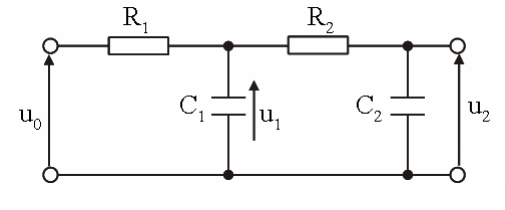
\includegraphics[scale=0.6]{czwornik.png}
                \caption{Schemat podwójnego czwórnika RC.}
            \end{figure}
        \item ogrzewanie centralne:
            \begin{itemize}
                \item ogrzewanie wody w rurach przez piec,
                \item przekazywanie ciepła za pomocą wody do grzejnika,
                \item ogrzewanie pomieszczenia poprzez grzejnik.
            \end{itemize}
        \item szeregowo podłączone elementy układu RLC.
    \end{itemize}
\end{document}
